\subsubsection{Модуль формирования и отправки приглашений}
В административной панели университета реализован отдельный модуль, который позволяет формировать и отправлять приглашения как для преподавателей, так и для студентов. Этот модуль работает по следующему сценарию:

\begin{enumerate}
    \item \textbf{Инициация приглашения:} 
    \begin{itemize}
        \item администратор вводит в UI адрес электронной почты и идентификатор кафедры (для приглашения преподавателя) либо адрес электронной почты и идентификатор группы (для приглашения студента),
        \item после заполнения необходимых полей администратор нажимает кнопку «Сформировать ссылку».
    \end{itemize}
    \item \textbf{Отправка запроса на бэкенд:} 
    \begin{itemize}
        \item UI передаёт запрос на бэкенд, например, «Запрос на приглашение преподавателя (требуются: email, department\_id)» или «Запрос на приглашение студента (требуются: email, group\_id)»,
        \item бэкенд проверяет права администратора и корректность введённых данных, генерирует уникальную ссылку приглашения и возвращает её обратно в UI.
    \end{itemize}
    \item \textbf{Получение ответа и отображение ссылки:} 
    \begin{itemize}
        \item UI получает от бэкенда объект с полем \texttt{invite\_link},
        \item UI отображает администратору уведомление «Приглашение отправлено» и показывает полученную ссылку, которую можно скопировать и отправить по электронной почте.
    \end{itemize}
\end{enumerate}

На рисунке~\ref{fig:admin-invite} приведена последовательная диаграмма, иллюстрирующая полный процесс формирования и отправки приглашений: в верхней части — сценарий для преподавателя, в нижней части — сценарий для студента.

\begin{figure}[H]
    \centering
    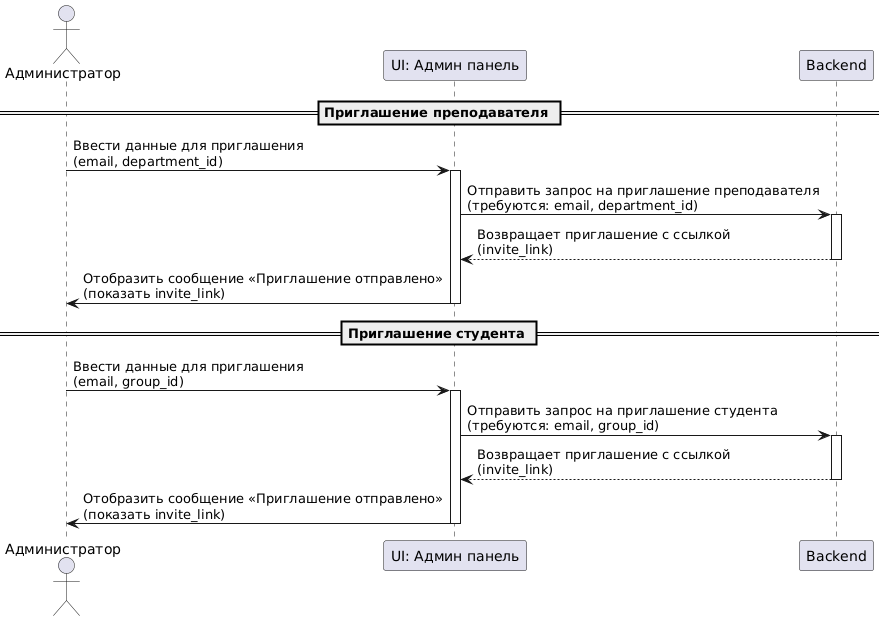
\includegraphics[width=0.9\textwidth]{static/diagrams/Admin.png}
    \caption{Схема процесса формирования и отправки приглашений преподавателям и студентам}
    \label{fig:admin-invite}
\end{figure}

На рисунке~\ref{fig:admin-invite} можно выделить следующие ключевые этапы:
\begin{itemize}
    \item \textbf{Приглашение преподавателя:}
    \begin{enumerate}
        \item администратор вводит в UI email и \texttt{department\_id},
        \item UI отправляет запрос на бэкенд «Приглашение преподавателя (требуются: email, department\_id)»,
        \item бэкенд проверяет данные, создаёт приглашение и возвращает уникальную ссылку (\texttt{invite\_link}),
        \item UI отображает сообщение «Приглашение отправлено» и показывает \texttt{invite\_link}.
    \end{enumerate}
    \item \textbf{Приглашение студента:}
    \begin{enumerate}
        \item администратор вводит в UI email и \texttt{group\_id},
        \item UI отправляет запрос на бэкенд «Приглашение студента (требуются: email, group\_id)»,
        \item бэкенд проверяет данные, создаёт приглашение и возвращает уникальную ссылку (\texttt{invite\_link}),
        \item UI отображает сообщение «Приглашение отправлено» и показывает \texttt{invite\_link}.
    \end{enumerate}
\end{itemize}

Таким образом, схема на рисунке~\ref{fig:admin-invite} демонстрирует единый алгоритм работы модуля: ввод данных в UI, отправка запроса на бэкенд, генерация и возврат уникальной ссылки, отображение ссылки администратору.
